% Бүлэг 1

\chapter{Proxy Re-Encryption схемийн онолын хэсэг} % Бүлгийн нэр
\label{Chapter1} % Энэ бүлэг рүү ишлэл хийх бол \ref{Chapter1} командыг ашигла 
\pagecolor{white}
%-------------------------------------------------------------------------------

% Агуулгад ашигласан хэвшүүлэлтийн зарим командын тодорхойлолт
\newcommand{\keyword}[1]{\textbf{#1}}
\newcommand{\tabhead}[1]{\textbf{#1}}
\newcommand{\code}[1]{\texttt{#1}}
\newcommand{\file}[1]{\texttt{\bfseries#1}}
\newcommand{\option}[1]{\texttt{\itshape#1}}

%-------------------------------------------------------------------------------
%	SECTION 1
%-------------------------------------------------------------------------------

\section{Өгөгдөл хуваалцах үйлчилгээ}
Өгөгдөл хуваалцах гэдэг нь өгөгдлийг программ болон хэрэглэгчид эсвэл байгуулгууд хоорондоо ашиглах боломжтой болгох үйл явц юм. Байгууллагын үр ашгийг нэмэгдүүлж, борлуулагчид болон түншүүдтэй хамтын ажиллагааг дэмжинэ. Хуваалцсан өгөгдлийн эрсдэл, боломжуудын талаар мэдлэгтэй байх нь үйл явцын салшгүй хэсэг юм.

%-------------------------------------------------------------------------------
%	SECTION 1
%-------------------------------------------------------------------------------

\section{Өгөгдөл аюулгүй байдал}


%-------------------------------------------------------------------------------
%	SECTION 1
%-------------------------------------------------------------------------------

\section{Шифрлэлт, түүний ач холбогдол, ангилал, хэрэглээ}
Мэдээллийн аюулгүй байдал үндсэн гурван зарчимыг тэнцвэртэй хангахыг зоридог. 
\begin{itemize}
    \item \textbf{Нууцлаг байдал (Confidentiality)}: Мэдээлэлийг нууц хэвээр нь хамгаалж үлдэх. Санаатай болон санамсаргүй мэдээллийг зөвшөөрөлгүй хуваалцах тараахаас сэргийлэх.
    \begin{itemize}
        \item Өгөгдлийн нууцлал (Data1 confidentiality)
        \item хувийн нууц (Privacy)
    \end{itemize}
    \item \textbf{Бүрэн бүтэн байдал (Integrity)}: Өгөгдөлд үнэн зөв найдвартай гадны нөлөө ороогүйг шалгах, бүрэн бүтэн хадаглах. 
    \begin{itemize}
        \item Өгөгдлийн бүрэн бүтэн байдал (Data integrity)
        \item Системийн бүрэн бүтэн байдал (System integrity) 
    \end{itemize}
    \item \textbf{Хүртээмжтэй байдал (Availability):} Тухайн системийн хэрэглэгчид хүртээмжтэй байх.
\end{itemize}

\begin{figure}[ht]
\centering
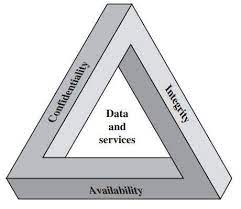
\includegraphics[scale=0.7]{Figures/cia_traid}
\caption[CIA гурвалжин]{CIA гурвалжин}
\label{fig:CIA}
\end{figure}

Криптографд шифрлэлт нь энгийн текстийг (жишээ нь, эх мессеж) шифр текст (жишээ нь, шифрлэгдсэн эсвэл кодлогдсон мессеж) болгон хувиргахад ашигладаг алгоритм юм. Шифрлэлтийн зорилго нь мессежийг түлхүүргүй хүн унших боломжгүй болгох явдал юм.

Мэдээлэл болон өгөгдлийг шифрлэлт хийснээр нууцлаг байдлыг хангах хамгийн том давуу тал юм. Бүрэн бүтэн байдал болон хүртээмжтэй байдлыг ч шифрлэлт нь хангах боломжтой.
Шифрлэлт ерөнхийд нь гурав ангилна.
\begin{itemize}
    \item \textbf{Тэгш хэмт шифрлэлт (symmetric)} нь шифрийг тайлах болон шифрлэхдээ нэг түлхүүр ашигладаг. Уламжлалт шифрлэлт гэх нь бий. Уламжлалт (компьютероос өмнөх үе) тэгш хэмтэй шифрүүд нь орлуулах эсвэл шилжүүлэх аргыг ашигладаг. Орлуулах арга нь энгийн текстийн элементүүд (тэмдэгтүүд, битүүд) шифр текстийн элементүүдэд солино оруулж тавина. Шилжүүлэх техник нь энгийн текстийн элементүүдийн байрлалыг системтэйгээр шилжүүлдэг. 
    Тэгш хэмт шифрлэлт нь хоёр төрөлтэй.
    \begin{itemize}
        \item Урсгал шифрлэлт (Stream шифрлэлт) RC4 болон ChaCha20 гэх мэт.
        \item Блок шифрлэлт (Block шифрлэлт) AES, DES, болон 3DES гэх мэт.
    \end{itemize}
    \item \textbf{Тэгш бус шифрлэлт (asymmetric)} нь нийтийн болон хувийн хоёр түлхүүртэй. Нийтийн түлхүүр нь нийтэд нээлтэй байдаг. Хувийн түлхүүрийг эмзэгшигч нь нууцалж алдахгүй байх ёстой. 
    \item \textbf{Хэш (Hash)} функц нь хувьсах урттай мессежийг тогтмол урттай хэш утга шифрлэдэг. Ихэнх хэш функц нь шахалтын алгоритм ашигладаг.
\end{itemize}

Криптограф нь дамжуулалтын явцад мессежийг хөндлөнгөөс өөрчлөлт ороогүй эсэхийг шалгаж бүрэн бүтэн байдлыг хангадаг. Хэш, мессежийг баталгаажуулалтын код (MACs), тоон гарын үсэг (Digital Signatures) ашигладаг байдаг.

\textbf{Мессежийн баталгаажуулалтын код (MACs)} нь авсан өгөгдөл нь илгээсэнтэй яг таарч (өөрчлөлт оруулах, устгах) мөн илгээгчийн баталгаажуулдаг.
Нууц түлхүүр ашигдаг. MAC нь хувьсах урттай мессежийг нууц түлхүүр болгон авч, баталгаажуулах код үүсгэдэг. MAC нь хэш функц болон тэгш хэмт блок шифрлэлтийг ашиглдаг.

\textbf{Тоон гарын үсэг (Digital Signatures)}

Ихэвчлэн шифрлэгдсэн мессэж, энгийн мессежийн хэшийг бүтээгчийн хувийн түлхүүрийн хэшийг авч харьцуулж баталгаажуулдаг.

%-------------------------------------------------------------------------------
%	SECTION 2
%-------------------------------------------------------------------------------

\section{Орчин үеийн ширфлэлтийн схемүүд}
Өгөгдлийг хэрхэн найдвартай нууцлаж хамгаалах нь чухал болсон. Зөвхөн шифрлэхээс гадна үүнийг схемчилж илүү хурдан өөр өөрсдийн давуу талтай схемүүдмйг хөгжүүлж гаргаж ирсэн.

\textbf{Танилтад суурилсан шифрлэлт (IBE)} 

Нийтийн түлхүүрийн оронд өөрийн хувийн мэдээллийг ашиглан өгөгдлийг шифрлэх, тайлах боломжийг олгодог нийтийн түлхүүрийн шифрлэлтийн нэг төрөл юм. IBE-ийг хэрэглэгчдийг таних тэмдэгээр нь мэддэг тохиолдолд аюулгүй өгөгдөл хуваалцахад ашиглаж болно.

\textbf{Шинж чанарт суурилсан шифрлэлэт (ABE)}

Энэ нь нас, албан тушаал, байгууллагын үүрэг зэрэг урьдчилан тодорхойлсон шинж чанарт үндэслэн өгөгдөлд хандах боломжийг олгодог шифрлэлтийн төрөл юм. ABE нь өгөгдөлд хандах хандалтыг нарийн хянахад ашиглагдаж болох ба зарим шинж чанарууд дээр үндэслэн хандалт олгосон хувилбаруудад ашиглаж болно.

\textbf{Гомоморф шифрлэлт (HE)}

Энэ нь шифрлэгдсэн өгөгдлийг эхлээд тайлахгүйгээр тооцоолол хийх боломжийг олгодог шифрлэлтийн төрөл юм. Тооцоолол хийх боломжийг олгохын зэрэгцээ өгөгдлийг нууцлах шаардлагатай тохиолдолд HE-г аюулгүй өгөгдөл боловсруулахад ашиглаж болно.

\textbf{Secure multiparty computation (MPC)}

Энэ талууд өөрсдийн оролтыг бие биедээ ил гаргахгүйгээр хувийн оролт дээрээ функцийг хамтран тооцоолох боломжийг олгодог криптографийн арга юм. Мэдээллийн нууцлалыг хадгалах, олон тал хамтран ажиллах шаардлагатай тохиолдолд MPC-ийг аюулгүй өгөгдөл боловсруулахад ашиглаж болно.

%-------------------------------------------------------------------------------
%	SECTION 3
%-------------------------------------------------------------------------------

\section{Proxy Re-Encryption схем}

Прокси дахин шифрлэлт нь нийтийн түлхүүрээр шифрлсэн өгөгдөлийг дахин ширфлэж өөр хувийн түлхүүрээр тайлах боломжийг олгодог.

Үндсэн хоёр төрөлтэй.
\begin{itemize}
    \item Нэг чиглэлт (Unidirectional PRE)
    \item Хоёр чиглэлт (Bidirectional PRE)
\end{itemize}

Нэг чиглэлт PRE (KE, RG, E, R, D) хэсгүүдээс тогтоно.

\begin{enumerate}
    \item Алис, Боб болон Чарли хувийн болон нийтийн түлхүүрийг үүсгэнэ. (KE)
    \item Алис Боб-д зориулж өгөгдлөө шифрлэж серверт байршуулна.
    \item Боб Алис-ын өгөгдлийг Чарли-тай хуваацлахын тулд RE(pkB,skB,pkC,skC∗) шифрлэж серверт байршуулна. Чарлигийн хувийн заавал шаардахгүй үүсгэж болно.
    \item Боб RE-г ашиглаж үүсэгсэн түлхүүрийг серверт явуулж Алисын файлыг дахин шифрлэж Чарли тайлах боломжтой болно.
\end{enumerate}

\begin{figure}[ht]
\centering
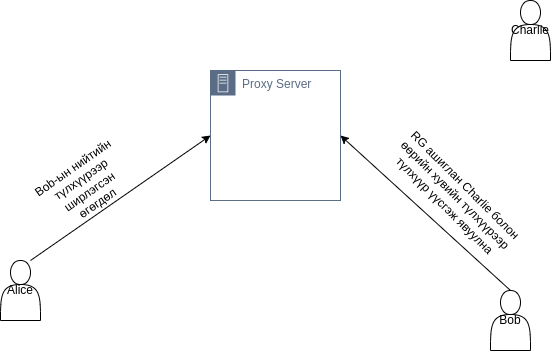
\includegraphics[scale=0.5]{Figures/pre}
\caption[Proxy Re-encryption scheme]{Proxy Re-encryption scheme}
\label{fig:PRE_Scheme}
\end{figure}

Давуу талууд:
\begin{itemize}
    \item Нууцлалыг сайжруулна: PRE нь оролцогч талуудын хувийн мэдээллийг задруулахгүйгээр өгөгдлийг хуваалцахыг зөвшөөрснөөр нууцлалыг сайжруулахад тусална. Энэ нь талууд нууцаар эсвэл хувийн нууц мэдээллийг задруулахгүйгээр мэдээллээ хуваалцахыг хүссэн тохиолдолд хэрэг болно.
    \item Нарийн төвөгтэй байдлыг багасгасан: PRE нь итгэмжлэгдсэн гуравдагч этгээдэд шифрлэлт болон шифрийг тайлах үйл явцыг удирдах боломжийг олгосноор шифрлэлт болон түлхүүрийн удирдлагын нарийн төвөгтэй байдлыг багасгахад тусална. Энэ нь ялангуяа олон талын оролцоотой, гол менежмент нь төвөгтэй, удирдахад хэцүү болж болзошгүй тохиолдолд хэрэг болно.
\end{itemize}

Сул талууд:
\begin{itemize}
    \item Проксид итгэх: PRE нь дахин шифрлэлтийг гүйцэтгхэд гуравдагч талын прокси дээр тулгуурладаг ба схемийн аюулгүй байдал нь прокси талаас хамаарна.
    \item Хязгаарлагдмал өргөтгөх чадвар: PRE нь өргөтгөх чадварын хувьд хязгаарлагдмал байж болно. Учир нь хэрэглэчдийн тоо нэмэгдэхийн хэрээр олон талыг дэмжихэд шаардлагатай дахин шифрлэлтийн түлхүүрүүдийн тоо хурдацтай өсөх болно. Энэ нь гол менежментийг төвөгтэй болгож, удирдахад хэцүү болгодог.
    \item Potential for replay attacks: PRE нь халдагч хариуг зогсоож хандах эрхийг өөрт ашигтай солих боломжтой. 
    \item Хүчингүй болгоход хүндрэлтэй байдал: PRE дахь өгөгдөлд хандах эрхийг цуцлах нь ялангуяа олон тал оролцсон тохиолдолд хэцүү байж болно. Хэрэв аль нэг талын дахин шифрлэлтийн түлхүүр алдагдсан бол бусад талуудын мэдээлэлд хандах эрхэд нөлөөлөхгүйгээр өгөгдөлд хандах эрхийг цуцлах нь хэцүү байж болно.
    \item Хязгаарлагдмал хэрэглээ: PRE нь харьцангуй шинэ бөгөөд шинээр гарч ирж буй технологи хэвээр байгаа бөгөөд илүү уламжлалт шифрлэлтийн схемүүдтэй харьцуулахад хэрэглээ нь хязгаарлагдмал байдаг. Энэ нь технологийг хэрэгжүүлэх, удирдах туршлагатай мэргэжилтнүүд бага байдаг.
\end{itemize}

%-------------------------------------------------------------------------------
%	SECTION 4
%-------------------------------------------------------------------------------

\section{Бүлгийн Дүгнэлт}
Энэ бүлэгт орчин үеийн шифрлэлтийн схеммүүдмйг судалж прокси дахин шифрлэлэт нь бусад схеммүүдээс ямар давуу тал сул талыг судалж харицуулсан. Системийн хөгжүүлэлт ерөнхий загварийг гаргаж юу хэрэгтэй сангуудыг ашиглан системийн хөгжүүлэлтыг хийж элсэн.